\documentclass{standalone}
\usepackage{tikz}
\usetikzlibrary{patterns, positioning}
\usepackage[sfdefault]{ClearSans} %% option 'sfdefault' activates Clear Sans as the default text font
\usepackage[T1]{fontenc}

\begin{document}
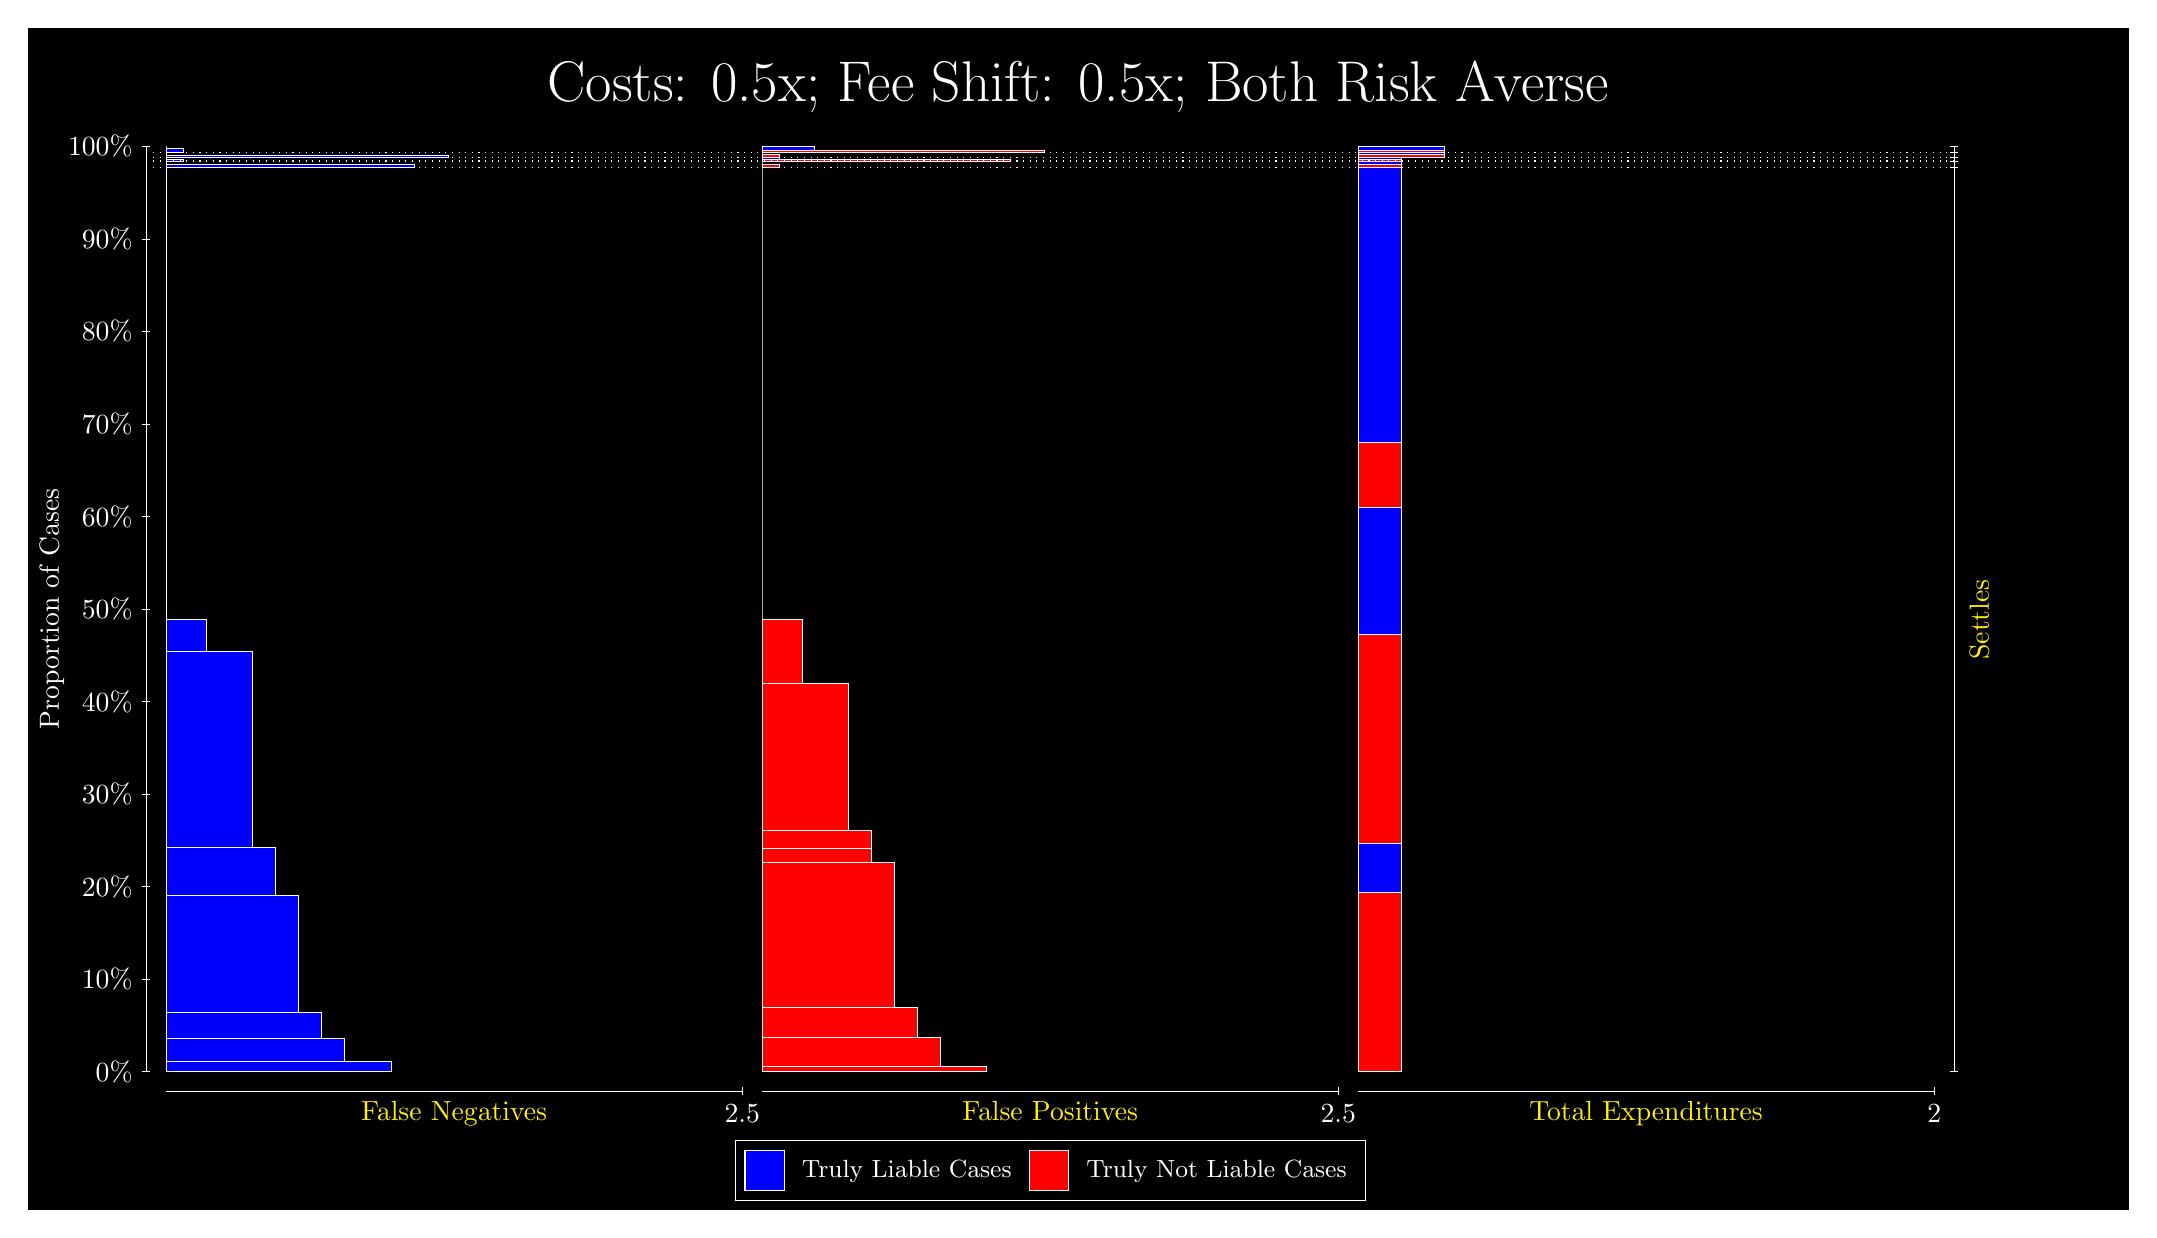
\begin{tikzpicture}
\draw[fill=black] (0,0) rectangle (26.667,15);
\draw[text=white] (0,13.5) rectangle (26.667,15) node[midway] {\huge Costs: 0.5x; Fee Shift: 0.5x; Both Risk Averse};
\draw[white, very thin] (1.5,1.75) -- (1.5,13.5);
\node[rotate=90, text=white, anchor=center] at (0.3, 7.625) {Proportion of Cases};
\draw[white, very thin] (1.45,1.75) -- (1.55,1.75);
\node[text=white, anchor=east] at (1.45, 1.75) {0\%};
\draw[white, very thin] (1.45,2.925) -- (1.55,2.925);
\node[text=white, anchor=east] at (1.45, 2.925) {10\%};
\draw[white, very thin] (1.45,4.1) -- (1.55,4.1);
\node[text=white, anchor=east] at (1.45, 4.1) {20\%};
\draw[white, very thin] (1.45,5.275) -- (1.55,5.275);
\node[text=white, anchor=east] at (1.45, 5.275) {30\%};
\draw[white, very thin] (1.45,6.45) -- (1.55,6.45);
\node[text=white, anchor=east] at (1.45, 6.45) {40\%};
\draw[white, very thin] (1.45,7.625) -- (1.55,7.625);
\node[text=white, anchor=east] at (1.45, 7.625) {50\%};
\draw[white, very thin] (1.45,8.8) -- (1.55,8.8);
\node[text=white, anchor=east] at (1.45, 8.8) {60\%};
\draw[white, very thin] (1.45,9.975) -- (1.55,9.975);
\node[text=white, anchor=east] at (1.45, 9.975) {70\%};
\draw[white, very thin] (1.45,11.15) -- (1.55,11.15);
\node[text=white, anchor=east] at (1.45, 11.15) {80\%};
\draw[white, very thin] (1.45,12.325) -- (1.55,12.325);
\node[text=white, anchor=east] at (1.45, 12.325) {90\%};
\draw[white, very thin] (1.45,13.5) -- (1.55,13.5);
\node[text=white, anchor=east] at (1.45, 13.5) {100\%};

\draw[white, very thin] (24.457,1.75) -- (24.457,13.5);
\draw[white, very thin] (24.407,1.75) -- (24.507,1.75);
\node[anchor=west] at (24.407, 1.75) {};
\draw[white, very thin] (24.407,13.233) -- (24.507,13.233);
\node[anchor=west] at (24.407, 13.233) {};
\draw[white, very thin] (24.407,13.314) -- (24.507,13.314);
\node[anchor=west] at (24.407, 13.314) {};
\draw[white, very thin] (24.407,13.358) -- (24.507,13.358);
\node[anchor=west] at (24.407, 13.358) {};
\draw[white, very thin] (24.407,13.427) -- (24.507,13.427);
\node[anchor=west] at (24.407, 13.427) {};
\draw[white, very thin] (24.407,13.5) -- (24.507,13.5);
\node[anchor=west] at (24.407, 13.5) {};

\draw[white, very thin, fill=blue] (1.75,1.75) rectangle (4.6044,1.8804);
\draw[white, very thin, fill=blue] (1.75,1.8804) rectangle (4.0188,2.1698);
\draw[white, very thin, fill=blue] (1.75,2.1698) rectangle (3.7261,2.5056);
\draw[white, very thin, fill=blue] (1.75,2.5056) rectangle (3.4333,3.9946);
\draw[white, very thin, fill=blue] (1.75,3.9946) rectangle (3.1406,4.6031);
\draw[white, very thin, fill=blue] (1.75,4.6031) rectangle (2.8478,7.0838);
\draw[white, very thin, fill=blue] (1.75,7.0838) rectangle (2.2623,7.4896);
\draw[white, very thin, fill=red] (1.75,7.4896) rectangle (1.75,13.233);
\draw[white, very thin, fill=blue] (1.75,13.233) rectangle (4.8971,13.269);
\draw[white, very thin, fill=red] (1.75,13.269) rectangle (1.75,13.314);
\draw[white, very thin, fill=blue] (1.75,13.314) rectangle (1.9696,13.34);
\draw[white, very thin, fill=red] (1.75,13.34) rectangle (1.75,13.358);
\draw[white, very thin, fill=blue] (1.75,13.358) rectangle (5.3362,13.383);
\draw[white, very thin, fill=red] (1.75,13.383) rectangle (1.75,13.427);
\draw[white, very thin, fill=blue] (1.75,13.427) rectangle (1.9696,13.475);
\draw[white, very thin, fill=red] (1.75,13.475) rectangle (1.75,13.5);
\draw[white, very thin, fill=red] (9.3189,1.75) rectangle (12.173,1.8149);
\draw[white, very thin, fill=red] (9.3189,1.8149) rectangle (11.588,2.1911);
\draw[white, very thin, fill=red] (9.3189,2.1911) rectangle (11.295,2.5703);
\draw[white, very thin, fill=red] (9.3189,2.5703) rectangle (11.002,4.404);
\draw[white, very thin, fill=red] (9.3189,4.404) rectangle (10.709,4.5807);
\draw[white, very thin, fill=red] (9.3189,4.5807) rectangle (10.709,4.8163);
\draw[white, very thin, fill=red] (9.3189,4.8163) rectangle (10.417,6.6808);
\draw[white, very thin, fill=red] (9.3189,6.6808) rectangle (9.8312,7.4936);
\draw[white, very thin, fill=blue] (9.3189,7.4936) rectangle (9.3189,13.233);
\draw[white, very thin, fill=red] (9.3189,13.233) rectangle (9.5384,13.278);
\draw[white, very thin, fill=blue] (9.3189,13.278) rectangle (9.3189,13.314);
\draw[white, very thin, fill=red] (9.3189,13.314) rectangle (12.466,13.332);
\draw[white, very thin, fill=blue] (9.3189,13.332) rectangle (9.5384,13.358);
\draw[white, very thin, fill=red] (9.3189,13.358) rectangle (9.5384,13.402);
\draw[white, very thin, fill=blue] (9.3189,13.402) rectangle (9.3189,13.427);
\draw[white, very thin, fill=red] (9.3189,13.427) rectangle (12.905,13.451);
\draw[white, very thin, fill=blue] (9.3189,13.451) rectangle (9.9776,13.5);
\draw[white, very thin, fill=red] (16.888,1.75) rectangle (17.437,4.0267);
\draw[white, very thin, fill=blue] (16.888,4.0267) rectangle (17.437,4.6519);
\draw[white, very thin, fill=red] (16.888,4.6519) rectangle (17.437,7.2985);
\draw[white, very thin, fill=blue] (16.888,7.2985) rectangle (17.437,8.9178);
\draw[white, very thin, fill=red] (16.888,8.9178) rectangle (17.437,9.7381);
\draw[white, very thin, fill=blue] (16.888,9.7381) rectangle (17.437,13.233);
\draw[white, very thin, fill=red] (16.888,13.233) rectangle (17.437,13.278);
\draw[white, very thin, fill=blue] (16.888,13.278) rectangle (17.437,13.314);
\draw[white, very thin, fill=red] (16.888,13.314) rectangle (17.437,13.332);
\draw[white, very thin, fill=blue] (16.888,13.332) rectangle (17.437,13.358);
\draw[white, very thin, fill=red] (16.888,13.358) rectangle (17.986,13.402);
\draw[white, very thin, fill=blue] (16.888,13.402) rectangle (17.986,13.427);
\draw[white, very thin, fill=red] (16.888,13.427) rectangle (17.986,13.451);
\draw[white, very thin, fill=blue] (16.888,13.451) rectangle (17.986,13.5);
\draw[white, dotted] (1.5,13.233) -- (24.457,13.233);
\draw[white, dotted] (1.5,13.314) -- (24.457,13.314);
\draw[white, dotted] (1.5,13.358) -- (24.457,13.358);
\draw[white, dotted] (1.5,13.427) -- (24.457,13.427);
\draw[white, very thin] (1.75,1.5) -- (9.0689,1.5);
\node[text=yellow, anchor=north] at (5.4094, 1.5) {False Negatives};
\draw[white, very thin] (9.0689,1.45) -- (9.0689,1.55);
\node[text=white, anchor=north] at (9.0689, 1.45) {2.5};

\draw[white, very thin] (9.3189,1.5) -- (16.638,1.5);
\node[text=yellow, anchor=north] at (12.978, 1.5) {False Positives};
\draw[white, very thin] (16.638,1.45) -- (16.638,1.55);
\node[text=white, anchor=north] at (16.638, 1.45) {2.5};

\draw[white, very thin] (16.888,1.5) -- (24.207,1.5);
\node[text=yellow, anchor=north] at (20.547, 1.5) {Total Expenditures};
\draw[white, very thin] (24.207,1.45) -- (24.207,1.55);
\node[text=white, anchor=north] at (24.207, 1.45) {2};

\node[text=yellow, centered, rotate=90] at (24.777, 7.4916) {Settles};





\draw (12.978300999999998,1.5) node[draw=none] (baseCoordinate) {};
\begin{scope}[align=center]
        \matrix[scale=0.5, draw=white, below=0.5cm of baseCoordinate, nodes={draw}, column sep=0.1cm]{
            \node[rectangle, draw, minimum width=0.5cm, minimum height=0.5cm, fill=blue] {}; &
            \node[draw=none, font=\small, text=white] (B) {Truly Liable Cases}; &
            \node[rectangle, draw, minimum width=0.5cm, minimum height=0.5cm, fill=red] {}; &
            \node[draw=none, font=\small, text=white] (B) {Truly Not Liable Cases}; \\
            };
\end{scope}

\end{tikzpicture}
\end{document}